\section{Image Processing Deep Neural Networks}\label{sec:image-processing-deep-neural-networks}

%Checked
\subsection{Overview of Convolutional Neural Networks}\label{subsec:convolutional-neural-networks}

CNNs constitute a class of deep learning models that are commonly used for computer vision tasks
including image classification, object detection, and semantic or instance segmentation.
Given the ability of convolutional neural networks to learn spatial hierarchies of features and their various types of data representations
(bounding box, segmentation mask, etc.), they are made ideal for the task of traffic object detection.
Many recent advances  in computer vision have been made possible by CNNs, including the development of models such as Yolo, Faster R-CNN, and SSD.
A dozen of these models have been developed, each with its own unique architecture and capabilities.
However, they all share the same fundamental principles gathered recently by Jiuxiang Gu in his 2018 work,
\("\)Recent advances in convolutional neural networks\("\)~\cite{GU2018354}.

The designation of the class is derived from the utilisation of convolutional layers,
which apply filters to the input data in order to extract features.
Additionally, convolutional neural networks comprise other layers, including
pooling layers, fully connected layers, and so forth.

These models are employed in a multitude of applications, including the perception
component in autonomous vehicles, surveillance systems, and medical imaging.
In view of the fact that these applications are in alignment with the project's stated objectives,
and given that the dataset in question is derived from a number of different urban traffic
environments, it has been decided that these types of neural networks should be employed for the
specific task of traffic object detection

The subsequent paragraphs will provide an overview of the essential components of convolutional neural networks.

\paragraph{Convolutional layers}\label{par:convolutional-layers}
represent the fundamental building blocks of convolutional neural networks.
Convolution operations are applied to the input data using filters (or in other word kernels) that process the input image.
This process enables the model to identify local patterns such as  edges, textures, and shapes.
Each convolutional layer generates a set of feature maps,
which indicate the presence of different types of these aforementioned features in the input.
These feature maps are then passed to the subsequent layers for further processing, such operations as pooling or classification,
to refine the information coded into the image.
During the training phase, the parameters of the kernels are learned (their values are adjusted), through backpropagation,
allowing the network to enhance feature extraction for specific tasks.


\begin{figure}[ht]
\centering
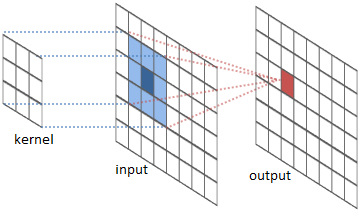
\includegraphics[width=.50\textwidth]{figures/convolution}
\caption{Convolutional layer operation~\cite{article}}
\label{fig:convolution}
\end{figure}

\paragraph{Fully connected layers}\label{par:fully-connected-layers}

is used to describe a type of neural network in which each
neuron is connected to every other neuron in the network's preceding layer, resulting in a dense connectivity pattern.
This connectivity pattern is also referred to as a "dense layer" due to its dense connections on the semantic figure.
They are typically located at the conclusion (HEAD) of convolutional neural network (CNN) architectures, where the final output is calculated.
In these layers, as one neuron receives data from every neuron in the previous layer, each connection characterised by a specific trainable weight and each neuron possesses a unique trainable bias.
This structure enables the model to integrate information from all features and make final predictions.
Fully connected layers in image processing or object detection tasks are computing the output probabilities for each class based on the features extracted by the preceding layers.
Regularization techniques, such as dropout and batch normalisation, are frequently employed in these layers to prevent overfitting.

Batch normalisation is a process that normalises the inputs of each layer in a neural network,
ensuring that their mean is zero and their standard deviation is one.
During training this normalisation is run on every mini-batch (small, randomly selected subset of training samples) of the data.

Dropout is a technique which involves the selecting of a random subset of neurons from the model's chosen layer, then ignoring them during training (dropping them out).
This results in their exclusion from the whole learning process.
The advantage of this process is that it helps the model to be resilient and less prone to overfitting, by forcing it to learn multiple independent representation of the data.

\begin{figure}[ht]
\centering
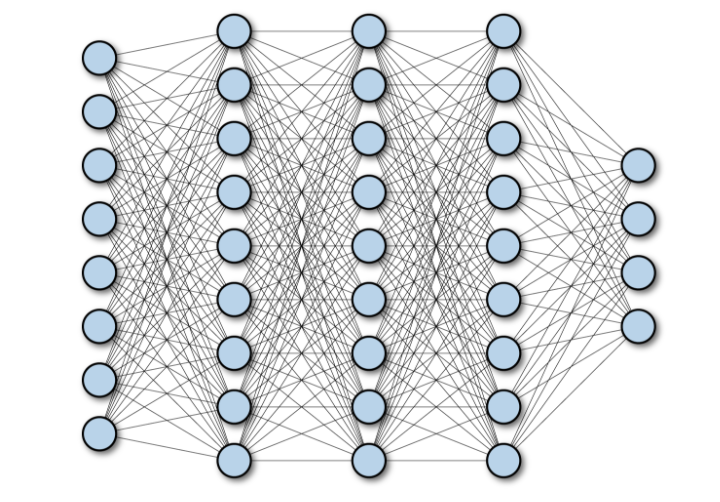
\includegraphics[width=0.50\textwidth]{figures/fully connected}
\caption{Fully Connected Layer semantics~\cite{article}}
\label{fig:fullconn}
\end{figure}


\subsubsection{Sampling layers}\label{subsub:sampling-layers}
Sampling layers are utilised to reduce the spatial dimensions of input data while maintaining its essential characteristics.
This process encompasses techniques such as sub-sampling,
strided convolutions, and global pooling.
The following section provides an in-depth examination of several frequently employed sampling methods.

In the following paragraphs I will discuss some of the most important sampling layers.

\paragraph{Max Pooling}
is one of the most prevalent sub-sampling techniques employed in convolutional neural networks.
In this approach, a sliding window processes the input feature map, and for each window,
the maximum value is selected. This operation reduces the dimensionality of the feature map,
preserving the most notable features (such as edges or textures) while discarding those of lesser relevance.
Max pooling is particularly effective in object detection tasks where maintaining the strongest activations is of paramount importance, as evidenced by the findings of GU.~\cite{GU2018354}.

\paragraph{Average Pooling}
, similarly to maximum pooling, average pooling utilises a sliding window; however, rather than
calculating the maximum value, it computes the average. This results in a more gradual
representation of the feature map and is frequently employed when the objective is to generalise
features to a greater extent than preserving sharp edges~\cite{GU2018354}.


\paragraph{Global Pooling}
methods, such as global max pooling and global average pooling, condense the entire feature map into a single value for each channel,
based on the method chosen, eg. if the global max pooling is chosen, entire channel is condensed into the maximal value of the channel.
This technique is commonly employed at the conclusion of a convolutional neural network, particularly in image classification tasks, where the spatial location of features is of lesser consequence than their mere presence. Global pooling mitigates the risk of overfitting by producing a compact representation of the input data, as evidenced by Ruby (2020).~\cite{GU2018354}.


\begin{figure}[h]
\centering
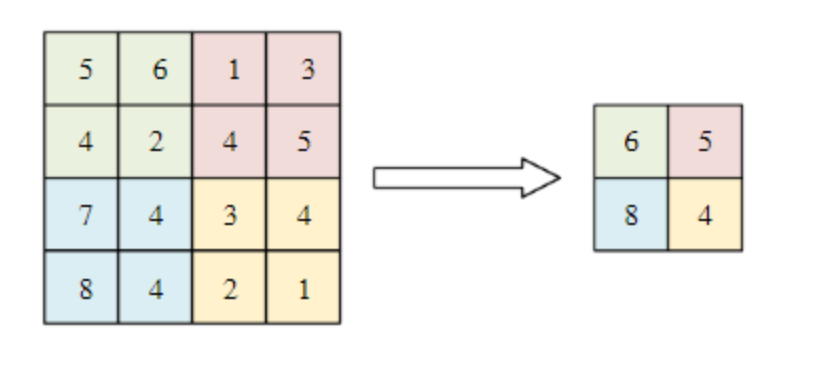
\includegraphics[width=.50\textwidth]{figures/pooling}
\caption{Pooling layer operation~\cite{article}}
\label{fig:pooling}
\end{figure}



\subsection{Activation Functions}\label{subsec:activation-functions}

Activation functions are employed in convolutional neural networks and other neural networks to introduce non-linearity into the model,
thereby enabling it to learn complex patterns and relationships within the data by determining the output of each neuron based on its input.
After calculating the weighted sum of the inputs to a neuron, the activation function transforms this sum into the output. These functions allows the model to represent a wide range of functions.
The output of the activation function serves as the input to the next layer.

In light of the work conducted by Siddharth Sharma and Simone Sharma regarding  activation functions~\cite{sharma2017activation}
the most prevalent  activation functions are ReLU, Sigmoid, and Tanh (Hyperbolic tangent).
Although alternative activation functions, such as BSF and ELU, could be employed, they are not utilised by the examined model (Yolov8).
Consequently, a detailed discussion of these functions will not be provided.
The following paragraphs  will discuss the ReLU, Sigmoid, and Tanh activation functions based on the work of Siddharth and Simone Sharma~\cite{sharma2017activation}.


\begin{figure}[h!]
    \centering


    \begin{subfigure}[b]{0.5\textwidth}
        \centering
        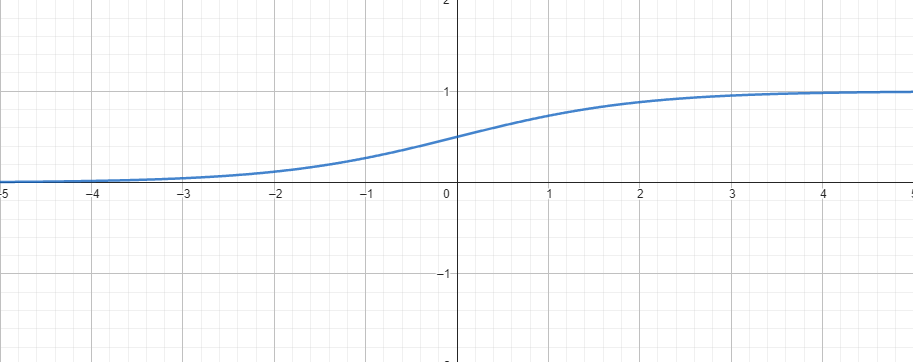
\includegraphics[width=\textwidth]{figures/sigmoid}
        \caption{Sigmoid activation function}
        \label{fig:sigmoid}
    \end{subfigure}
    \hfill
    \begin{subfigure}[b]{0.45\textwidth}
        \centering
        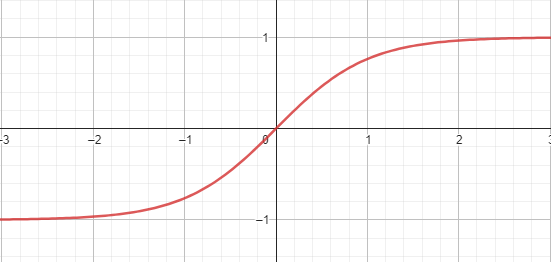
\includegraphics[width=\textwidth]{figures/tanh}
        \caption{Tanh activation function}
        \label{fig:tanh}
    \end{subfigure}
    \hfill
    \begin{subfigure}[b]{0.45\textwidth}
        \centering
        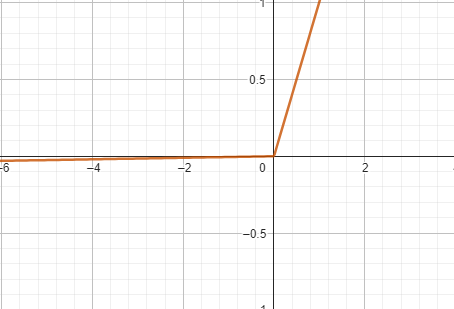
\includegraphics[width=\textwidth]{figures/relu}
        \caption{ReLU activation function}
        \label{fig:relu}
    \end{subfigure}

    \caption{Activation functions: Sigmoid,Tanh and ReLU}
    \label{fig:activation_functions}
\end{figure}


\paragraph{ReLU:}\label{par:relu}
the Rectified Linear Unit (ReLU) is one of the most common and easy to understand activation functions in convolutional (or any other) neural networks.
It is defined as \( f(x) = \max(0, x) \) in the works of Siddharth Sharma~\cite{sharma2017activation}.
This function introduces non-linearity while maintaining a simple and efficient computation.
The ReLU function helps mitigate the vanishing gradient issue, allowing models to learn faster and perform better.
However, be susceptible to the phenomenon known as the \("\)dying ReLU\("\) problem, where neurons become inactive and only output zeros,
particularly during the training of deep networks.



\paragraph{Sigmoid:}\label{par:sigmoid}
the Sigmoid function translates input values to a range between 0 and 1,
rendering it useful for binary classification problems.
It is defined as \( f(x) = \frac{1}{1 + e^{-x}} \) in the works of Siddharth Sharma~\cite{sharma2017activation}.
While the Sigmoid function provides smooth gradients,
it is prone to the vanishing gradient problem,
especially for large positive or negative input values.
This can slow down the training of deep networks,
which is why it is often replaced by other activation
functions in hidden layers,
though it still finds use in the output layer for binary classification tasks.



\paragraph{Tanh:}\label{par:tanh}
the hyperbolic tangent (Tanh) function is another activation function that maps input values to a range between -1 and 1.
It is defined as  \( f(x) = \frac{e^x - e^{-x}}{e^x + e^{-x}} \)in the works of Siddharth Sharma~\cite{sharma2017activation}.
The Tanh function is zero-centered and centricaly symmetrical, facilitates the centring of the data and may result in accelerated convergence during training.
Nevertheless, it continues to exhibit the vanishing gradient problem for large input values, though to a lesser extent than the Sigmoid function.



\subsection{Introduction to YOLO}\label{subsec:introduction-to-yolo}

The YOLO (You Only Look Once) model is a relatively recent object detection system that is straightforward to utilise and comprehend, while also benefiting from a thriving community of users and developers.
It is based on the YOLO algorithm, which is a real-time object detection algorithm developed by Joseph Redmon and Ali Farhadi in 2015\cite{redmon2016lookonceunifiedrealtime}.



Unlike traditional object detection methods that apply classifiers to various sections of an image,
YOLO (You Only Look Once) approaches the problem as a single regression problem.
The algorithm divides the input image into an
\(S \times S\) grid and predicts bounding boxes and class probabilities in parallel for each grid cell,
enabling the model to detect multiple types and instances of objects in a single run.
This kind of architecture not only enhances speed by processing the entire image at once
but also improves detection accuracy by reducing the number of false positives.
By minimizing redundant detections and effectively capturing the spatial context of objects,
YOLO allows for real-time applications, given its fast inference speeds, making it particularly effective in scenarios such as video surveillance, autonomous driving, and robotics.

The YOLO model has evolved through multiple versions, with improvements in both performance and varying capability.
Subsequent versions of the model, including Yolov2, Yolov3, and the latest Yolov5 and Yolov7, as well as Yolov8 (with Yolov10 and 11 forthcoming),
have introduced advancements in network architecture,
feature extraction, and training techniques.
These developments have rendered YOLO a suitable candidate for a noumber of applications,
including autonomous vehicles, as evidenced by my own observations during my work in the industry, surveillance systems, and real-time video analysis.

A further noteworthy attribute of the Yolo-type neural networks is their scalability and versatility in terms of model architecture.
These models are available in a range of sizes (\textit{nano, small, medium, large, extralarge}) and with a variety of detection types (\textit{semantic segmentation, bounding boxes,
oriented bounding boxes, instance segmentation}), which can be deployed in diverse scenarios.




\begin{figure}[ht]
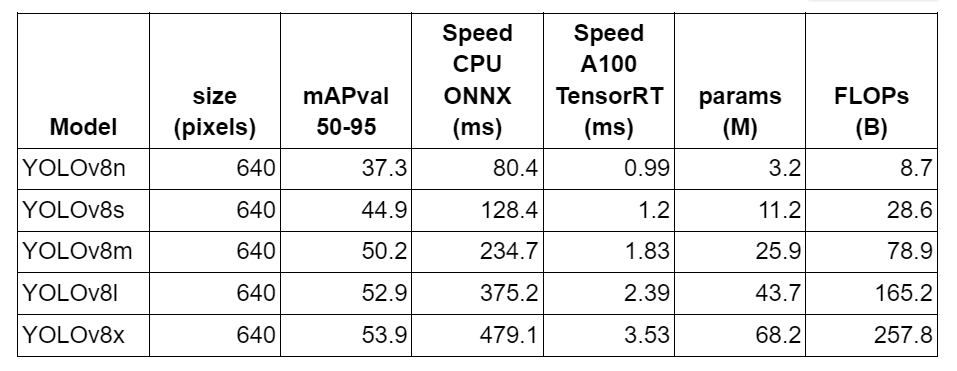
\includegraphics[width=1.0\textwidth]{figures/table1}
\caption{Different sizes of the Yolov8~\cite{githubGitHubUltralyticsultralytics}}
\label{fig:tableofsizes}
\end{figure}

\subsubsection{The role of model size}\label{subsubsec:model-size}
In the field of computer vision, particularly in the context of object detection tasks, the selection of an appropriate size for a
Yolov8 model, such as Yolov8-Nano, Yolov8-Small,Yolov8-Medium,  Yolov8-Large, or Yolov8-eXtra-large is of paramount importance in order to achieve an optimal balance between accuracy, speed, and resource efficiency.

The smaller models are lightweight and operate at high speeds, rendering them optimal for real-time applications on devices with constrained computational capabilities, such as mobile phones or edge devices.
Although they consume less memory and processing power, they may compromise some accuracy, which can be an acceptable trade-off in applications where speed is more important than precision.

In contrast, larger models demonstrate superior accuracy and are capable of handling intricate image details with greater precision, trough the models large number of trainable and frozen(not trainable) parameters.
They are better suited to scenarios where there are fewer computational constraints, such as high-powered GPUs or cloud environments, where precise detection is essential.

Selecting an appropriate model size allows developers to tailor solutions to the specific needs of their applications, ensuring both cost-effectiveness and reliability.
This careful selection directly influences the efficiency and effectiveness of computer vision systems, optimising them for diverse deployment environments.

In light of these considerations, I have opted to utilise a medium-sized model, aiming to strike a balance between computational capacity and accuracy.

\subsection{Model architecture}\label{subsec:architecture}
This network, like many others in the CNN family, has a distinctive architectural configuration that
enables the execution of intricate tasks such as object detection and classification.
The system is constituted of three distinct and discrete components,
each comprising a unique set of layers that perform specific and separate functions.
The following paragraphs aim to provide an overview of these elements and their contribution to the model's detection.

\begin{figure}[ht]
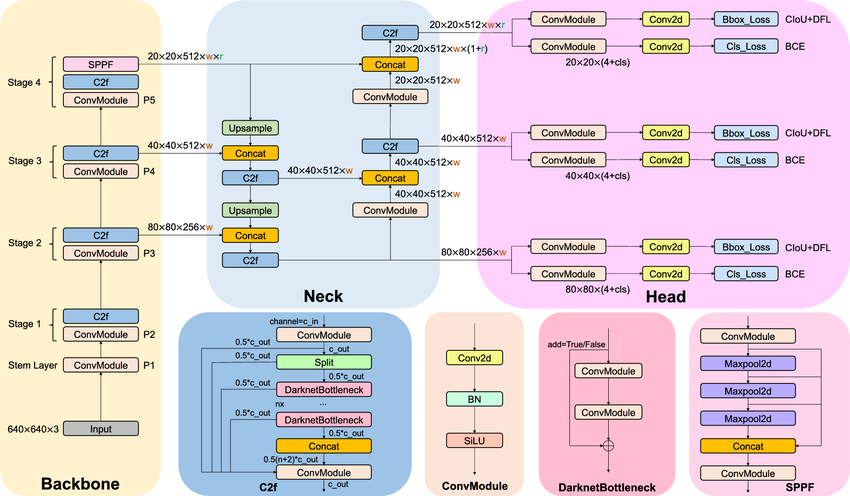
\includegraphics[width=1.0\textwidth]{figures/Detailed-illustration-of-YOLOv8-model-architecture-The-Backbone-Neck-and-Head-are-the}
\caption{The architecture of the Yolov8 model~\cite{FractureDetection2024}}
\label{fig:architecture}
\end{figure}
\newpage
\paragraph{Backbone:}\label{par:backbone}
the Yolov8 model is based on convolutional neural networks that have been specifically designed to capture essential features from input images.
It comprises multiple layers of convolutional operations (called Conv and a complex layer called C2F)
that extract progressively more sophisticated representations.
This structure emphasises both depth and computational efficiency,
enabling the model to discern subtle details while maintaining rapid processing capabilities.
Innovations such as skip connections and normalization techniques are employed to enhance the learning dynamics and improve the model's robustness to variations in input conditions.
%kép a backbone-ról

\paragraph{Neck:}\label{par:neck}
in the Yolov8 architectural design, the neck serves as an intermediary between the backbone and the head.
The primary function of the neck is to consolidate features from the various levels of the backbone,
thereby enhancing the model's ability to detect objects across different scales.
By employing strategies such as feature fusion or pyramid pooling,
the neck effectively integrates both coarse and fine features,
enabling the model to better handle overlapping objects and diverse scene contexts.
This feature aggregation is crucial for optimising the detection performance,
as it allows the model to harness a comprehensive range of information.

\newpage
\paragraph{Head:}\label{par:head}
the head of the Yolov8 model is responsible for generating the final outputs,
which are based on the features that have been processed through the neck.
The final stage of the Yolov8 model translates the aggregated feature maps into bounding box predictions and associated class scores for each detected object.
This section typically employs a combination of convolutional and fully connected layers to refine these outputs,
ensuring they are accurate and meaningful.
Additionally, the head may implement techniques such as adaptive anchors or
confidence scoring to enhance the localisation and classification accuracy.
By effectively synthesising the rich feature information, the head enables Yolov8 to achieve high-performance object detection suitable for a wide array of applications.

%kép a headről
\subsection{Training}\label{subsec:training}
The training process~\cite{redmon2016lookonceunifiedrealtime} for the Yolov8 model involves feeding its input with a large dataset of labelled images.
The model learns to identify objects by minimizing the difference between its predictions and the actual labels trough multiple iterations:
After a training cycle, if the default settings are kept, a validation function (so called \("\)val\("\))\ is run,
to determine more information on the model's performance on pictures that are not present in the training set.
The training process is iterative, with the model adjusting its parameters to improve its predictions over time.
This process is computationally intensive and requires access to powerful hardware,
the best fitting hardware for this purpose, that can be found in an ordinary PC, is the GPU\@.

The training process involves several key steps, including data preprocessing, model initialization,
loss calculation, and parameter optimization.
The model is trained using a technique called backpropagation, which involves adjusting the model's weights based on
the error between its predictions and the ground truth labels.

The Yolov8 model uses a number of different loss functions, according to the original paper~\cite{redmon2016lookonceunifiedrealtime}
, loss functions to measure the difference between its predictions and the actual labels in different ways:
\newpage


\begin{itemize}
\item \textbf{CIoU (Complete Intersection over Union) loss}:
\begin{equation}
\text{CIoU} = 1 - \left( \text{IoU} - \frac{\rho^2(\mathbf{b}, \mathbf{b}^g)}{c^2} - \alpha v \right) ~\cite{li2020generalizedfocallosslearning}\label{eq:equation3}
\end{equation}
where \(\rho\) is the Euclidean distance between the centre-points of the predicted box \(\mathbf{b}\) and
 the ground truth box \(\mathbf{b}^g\), \(c\) is the diagonal length of the smallest enclosing box covering
 the two boxes, \(\alpha\) is a positive trade-off parameter that serves to balance the importance of the aspect ratio consistency term \(v\),  that measures the consistency of aspect
 ratios.
 It is more sensible to localisation accuracy.

\item \textbf{DFL (Distribution Focal Loss)}:
\begin{equation}
\text{DFL} = -\sum_{i=1}^{N} p_i \log(q_i)~\cite{DBLP:journals/corr/abs-1911-08287}\label{eq:equation2}
\end{equation}
where \(p_i\) is the true probability distribution and \(q_i\) is the predicted probability distribution.
It is sensible to the accuracy classification.
\item \textbf{BCE (binary cross-entropy for classification loss)}:
\begin{equation}
\text{BCE} = -\sum_{i=1}^{N} y_i \log(p_i) + (1 - y_i) \log(1 - p_i)~\cite{ruby2020binary}\label{eq:equation}
\end{equation}
where \(y_i\) is the true label and \(p_i\) is the predicted probability.

\end{itemize}



I opted for training the model on my local machine, using a single GPU, while it provided me with sufficient performance, the training time was significantly longer than it would have been on a more powerful cloud machine.
To reduce the chance of overfitting, the training dataset is typically divided into training and validation sets,
with the latter used to evaluate the model's performance on unseen data.
The trainings batch size where set to 3, which is not common, but it was necessary to fit the model on the GPU,
to optimise training time.

\newpage